% Options for packages loaded elsewhere
\PassOptionsToPackage{unicode}{hyperref}
\PassOptionsToPackage{hyphens}{url}
%
\documentclass[
  12pt,
]{article}
\usepackage{amsmath,amssymb}
\usepackage{lmodern}
\usepackage{ifxetex,ifluatex}
\ifnum 0\ifxetex 1\fi\ifluatex 1\fi=0 % if pdftex
  \usepackage[T1]{fontenc}
  \usepackage[utf8]{inputenc}
  \usepackage{textcomp} % provide euro and other symbols
\else % if luatex or xetex
  \usepackage{unicode-math}
  \defaultfontfeatures{Scale=MatchLowercase}
  \defaultfontfeatures[\rmfamily]{Ligatures=TeX,Scale=1}
\fi
% Use upquote if available, for straight quotes in verbatim environments
\IfFileExists{upquote.sty}{\usepackage{upquote}}{}
\IfFileExists{microtype.sty}{% use microtype if available
  \usepackage[]{microtype}
  \UseMicrotypeSet[protrusion]{basicmath} % disable protrusion for tt fonts
}{}
\makeatletter
\@ifundefined{KOMAClassName}{% if non-KOMA class
  \IfFileExists{parskip.sty}{%
    \usepackage{parskip}
  }{% else
    \setlength{\parindent}{0pt}
    \setlength{\parskip}{6pt plus 2pt minus 1pt}}
}{% if KOMA class
  \KOMAoptions{parskip=half}}
\makeatother
\usepackage{xcolor}
\IfFileExists{xurl.sty}{\usepackage{xurl}}{} % add URL line breaks if available
\IfFileExists{bookmark.sty}{\usepackage{bookmark}}{\usepackage{hyperref}}
\hypersetup{
  pdftitle={Your title},
  hidelinks,
  pdfcreator={LaTeX via pandoc}}
\urlstyle{same} % disable monospaced font for URLs
\usepackage{longtable,booktabs,array}
\usepackage{calc} % for calculating minipage widths
% Correct order of tables after \paragraph or \subparagraph
\usepackage{etoolbox}
\makeatletter
\patchcmd\longtable{\par}{\if@noskipsec\mbox{}\fi\par}{}{}
\makeatother
% Allow footnotes in longtable head/foot
\IfFileExists{footnotehyper.sty}{\usepackage{footnotehyper}}{\usepackage{footnote}}
\makesavenoteenv{longtable}
\usepackage{graphicx}
\makeatletter
\def\maxwidth{\ifdim\Gin@nat@width>\linewidth\linewidth\else\Gin@nat@width\fi}
\def\maxheight{\ifdim\Gin@nat@height>\textheight\textheight\else\Gin@nat@height\fi}
\makeatother
% Scale images if necessary, so that they will not overflow the page
% margins by default, and it is still possible to overwrite the defaults
% using explicit options in \includegraphics[width, height, ...]{}
\setkeys{Gin}{width=\maxwidth,height=\maxheight,keepaspectratio}
% Set default figure placement to htbp
\makeatletter
\def\fps@figure{htbp}
\makeatother
\setlength{\emergencystretch}{3em} % prevent overfull lines
\providecommand{\tightlist}{%
  \setlength{\itemsep}{0pt}\setlength{\parskip}{0pt}}
\setcounter{secnumdepth}{5}
\usepackage[a4paper, total={6in, 8in}]{geometry}
\usepackage{booktabs}
\usepackage{float}
\usepackage{setspace}\doublespacing
\usepackage{lineno}
\linenumbers
\usepackage{fontspec}
\usepackage{multirow}
\usepackage{multicol}
\usepackage{colortbl}
\usepackage{hhline}
\usepackage{longtable}
\usepackage{array}
\usepackage{hyperref}
\ifluatex
  \usepackage{selnolig}  % disable illegal ligatures
\fi
\newlength{\cslhangindent}
\setlength{\cslhangindent}{1.5em}
\newlength{\csllabelwidth}
\setlength{\csllabelwidth}{3em}
\newenvironment{CSLReferences}[2] % #1 hanging-ident, #2 entry spacing
 {% don't indent paragraphs
  \setlength{\parindent}{0pt}
  % turn on hanging indent if param 1 is 1
  \ifodd #1 \everypar{\setlength{\hangindent}{\cslhangindent}}\ignorespaces\fi
  % set entry spacing
  \ifnum #2 > 0
  \setlength{\parskip}{#2\baselineskip}
  \fi
 }%
 {}
\usepackage{calc}
\newcommand{\CSLBlock}[1]{#1\hfill\break}
\newcommand{\CSLLeftMargin}[1]{\parbox[t]{\csllabelwidth}{#1}}
\newcommand{\CSLRightInline}[1]{\parbox[t]{\linewidth - \csllabelwidth}{#1}\break}
\newcommand{\CSLIndent}[1]{\hspace{\cslhangindent}#1}

\title{Your title}
\author{}
\date{\vspace{-2.5em}}

\begin{document}
\maketitle

Name\textsuperscript{1}, Name\textsuperscript{2}. \newline

\textsuperscript{1}Affiliation, \newline
\textsuperscript{2}Affiliation. \newline

\textbf{keywords:} words. \newline

\textbf{Correspondence:} \newline
Name \newline
\href{mailto:email@email.com}{\nolinkurl{email@email.com}} \newline

\pagebreak

\hypertarget{abstract}{%
\section*{Abstract}\label{abstract}}
\addcontentsline{toc}{section}{Abstract}

Write your abstract

\pagebreak

\hypertarget{intro}{%
\section{Introduction}\label{intro}}

Write your introduction

Examples of some citation formats:

(\protect\hyperlink{ref-Darwin1859}{Darwin 1859})

\protect\hyperlink{ref-Bumpus1898}{Bumpus} (\protect\hyperlink{ref-Bumpus1898}{1898})

(\protect\hyperlink{ref-Darwin1859}{Darwin 1859}; \protect\hyperlink{ref-Bumpus1898}{Bumpus 1898})

(e.g., \protect\hyperlink{ref-Bumpus1898}{Bumpus 1898})

\hypertarget{methods}{%
\section{Methods}\label{methods}}

\begin{align}
t = \frac{\bar{X}_{1} - \bar{X}_{2}} {s_{p} \times \sqrt{\frac{1}{n_{1}} + \frac{1}{n_{2}}}} \label{eq:H1S}
\end{align}

In equation \eqref{eq:H1S}, \(\bar{X}_{1}\) and \(\bar{X}_{2}\) are the mean of the samples. Similarly, \(n_{1}\) and \(n_{2}\) are the sample sizes, and \(s_{p}\).

\hypertarget{results}{%
\section{Results}\label{results}}

The mean value of group x (126.27) was larger than the mean value of group y (112.68; t: 3.65, p: \ensuremath{7.97\times 10^{-4}}).

Cross-reference to Fig. \ref{fig:fig1}.

Cross-reference to Table \ref{tab:tab1}.

\hypertarget{discussion}{%
\section{Discussion}\label{discussion}}

Write your discussion

\hypertarget{conclusion}{%
\section{Conclusion}\label{conclusion}}

Write your conclusion

\pagebreak

\hypertarget{acknowledgment}{%
\section*{Acknowledgment}\label{acknowledgment}}
\addcontentsline{toc}{section}{Acknowledgment}

\hypertarget{orcid-ids}{%
\section*{ORCID ids}\label{orcid-ids}}
\addcontentsline{toc}{section}{ORCID ids}

\pagebreak

\hypertarget{references}{%
\section*{References}\label{references}}
\addcontentsline{toc}{section}{References}

\hypertarget{refs}{}
\begin{CSLReferences}{1}{0}
\leavevmode\hypertarget{ref-Bumpus1898}{}%
Bumpus, H. C. 1898. {Eleventh lecture. The elimination of the unfit as illustrated by the introduced sparrow, {\emph{Passer domesticus}}. (A fourth contribution to the study of variation.)}. Biological Lectures: Woods Hole Marine Biological Laboratory 209--225.

\leavevmode\hypertarget{ref-Darwin1859}{}%
Darwin, C. 1859. {The Origin of Species}. Penguin, New York.

\end{CSLReferences}

\pagebreak

\hypertarget{figures}{%
\section*{Figures}\label{figures}}
\addcontentsline{toc}{section}{Figures}

\begin{figure}[H]
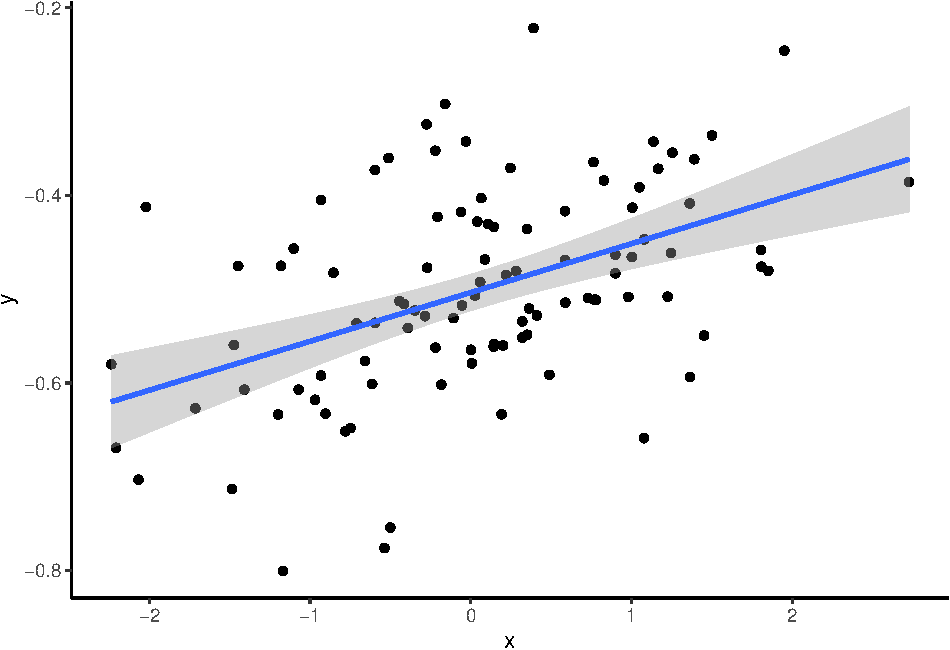
\includegraphics[width=1\linewidth]{_main_files/figure-latex/fig1-1} \caption{Figure caption}\label{fig:fig1}
\end{figure}

\pagebreak

\hypertarget{tables}{%
\section*{Tables}\label{tables}}
\addcontentsline{toc}{section}{Tables}

\providecommand{\docline}[3]{\noalign{\global\setlength{\arrayrulewidth}{#1}}\arrayrulecolor[HTML]{#2}\cline{#3}}

\setlength{\tabcolsep}{2pt}

\renewcommand*{\arraystretch}{1.5}

\begin{longtable}[c]{|p{0.40in}|p{0.50in}}

\caption{My table caption}\label{tab:tab1}\\

\hhline{>{\arrayrulecolor[HTML]{666666}\global\arrayrulewidth=2pt}->{\arrayrulecolor[HTML]{666666}\global\arrayrulewidth=2pt}-}

\multicolumn{1}{!{\color[HTML]{000000}\vrule width 0pt}>{\raggedleft}p{\dimexpr 0.4in+0\tabcolsep+0\arrayrulewidth}}{\fontsize{11}{11}\selectfont{\textcolor[HTML]{000000}{\global\setmainfont{Arial}id}}} & \multicolumn{1}{!{\color[HTML]{000000}\vrule width 0pt}>{\raggedright}p{\dimexpr 0.5in+0\tabcolsep+0\arrayrulewidth}!{\color[HTML]{000000}\vrule width 0pt}}{\fontsize{11}{11}\selectfont{\textcolor[HTML]{000000}{\global\setmainfont{Arial}res}}} \\

\noalign{\global\setlength{\arrayrulewidth}{2pt}}\arrayrulecolor[HTML]{666666}\cline{1-2}

\endfirsthead

\hhline{>{\arrayrulecolor[HTML]{666666}\global\arrayrulewidth=2pt}->{\arrayrulecolor[HTML]{666666}\global\arrayrulewidth=2pt}-}

\multicolumn{1}{!{\color[HTML]{000000}\vrule width 0pt}>{\raggedleft}p{\dimexpr 0.4in+0\tabcolsep+0\arrayrulewidth}}{\fontsize{11}{11}\selectfont{\textcolor[HTML]{000000}{\global\setmainfont{Arial}id}}} & \multicolumn{1}{!{\color[HTML]{000000}\vrule width 0pt}>{\raggedright}p{\dimexpr 0.5in+0\tabcolsep+0\arrayrulewidth}!{\color[HTML]{000000}\vrule width 0pt}}{\fontsize{11}{11}\selectfont{\textcolor[HTML]{000000}{\global\setmainfont{Arial}res}}} \\

\noalign{\global\setlength{\arrayrulewidth}{2pt}}\arrayrulecolor[HTML]{666666}\cline{1-2}\endhead



\multicolumn{1}{!{\color[HTML]{000000}\vrule width 0pt}>{\raggedleft}p{\dimexpr 0.4in+0\tabcolsep+0\arrayrulewidth}}{\fontsize{11}{11}\selectfont{\textcolor[HTML]{000000}{\global\setmainfont{Arial}1}}} & \multicolumn{1}{!{\color[HTML]{000000}\vrule width 0pt}>{\raggedright}p{\dimexpr 0.5in+0\tabcolsep+0\arrayrulewidth}!{\color[HTML]{000000}\vrule width 0pt}}{\fontsize{11}{11}\selectfont{\textcolor[HTML]{000000}{\global\setmainfont{Arial}a}}} \\





\multicolumn{1}{!{\color[HTML]{000000}\vrule width 0pt}>{\raggedleft}p{\dimexpr 0.4in+0\tabcolsep+0\arrayrulewidth}}{\fontsize{11}{11}\selectfont{\textcolor[HTML]{000000}{\global\setmainfont{Arial}2}}} & \multicolumn{1}{!{\color[HTML]{000000}\vrule width 0pt}>{\raggedright}p{\dimexpr 0.5in+0\tabcolsep+0\arrayrulewidth}!{\color[HTML]{000000}\vrule width 0pt}}{\fontsize{11}{11}\selectfont{\textcolor[HTML]{000000}{\global\setmainfont{Arial}b}}} \\





\multicolumn{1}{!{\color[HTML]{000000}\vrule width 0pt}>{\raggedleft}p{\dimexpr 0.4in+0\tabcolsep+0\arrayrulewidth}}{\fontsize{11}{11}\selectfont{\textcolor[HTML]{000000}{\global\setmainfont{Arial}3}}} & \multicolumn{1}{!{\color[HTML]{000000}\vrule width 0pt}>{\raggedright}p{\dimexpr 0.5in+0\tabcolsep+0\arrayrulewidth}!{\color[HTML]{000000}\vrule width 0pt}}{\fontsize{11}{11}\selectfont{\textcolor[HTML]{000000}{\global\setmainfont{Arial}c}}} \\





\multicolumn{1}{!{\color[HTML]{000000}\vrule width 0pt}>{\raggedleft}p{\dimexpr 0.4in+0\tabcolsep+0\arrayrulewidth}}{\fontsize{11}{11}\selectfont{\textcolor[HTML]{000000}{\global\setmainfont{Arial}4}}} & \multicolumn{1}{!{\color[HTML]{000000}\vrule width 0pt}>{\raggedright}p{\dimexpr 0.5in+0\tabcolsep+0\arrayrulewidth}!{\color[HTML]{000000}\vrule width 0pt}}{\fontsize{11}{11}\selectfont{\textcolor[HTML]{000000}{\global\setmainfont{Arial}d}}} \\





\multicolumn{1}{!{\color[HTML]{000000}\vrule width 0pt}>{\raggedleft}p{\dimexpr 0.4in+0\tabcolsep+0\arrayrulewidth}}{\fontsize{11}{11}\selectfont{\textcolor[HTML]{000000}{\global\setmainfont{Arial}5}}} & \multicolumn{1}{!{\color[HTML]{000000}\vrule width 0pt}>{\raggedright}p{\dimexpr 0.5in+0\tabcolsep+0\arrayrulewidth}!{\color[HTML]{000000}\vrule width 0pt}}{\fontsize{11}{11}\selectfont{\textcolor[HTML]{000000}{\global\setmainfont{Arial}e}}} \\

\noalign{\global\setlength{\arrayrulewidth}{2pt}}\arrayrulecolor[HTML]{666666}\cline{1-2}

\end{longtable}

\pagebreak

\hypertarget{supplementaty-materials}{%
\section*{Supplementaty materials}\label{supplementaty-materials}}
\addcontentsline{toc}{section}{Supplementaty materials}

\renewcommand{\thefigure}{S\arabic{figure}}
\setcounter{figure}{0}
\renewcommand{\thetable}{S\arabic{table}}
\setcounter{table}{0}
\renewcommand{\theequation}{S\arabic{equation}}
\setcounter{equation}{0}

\begin{figure}[H]
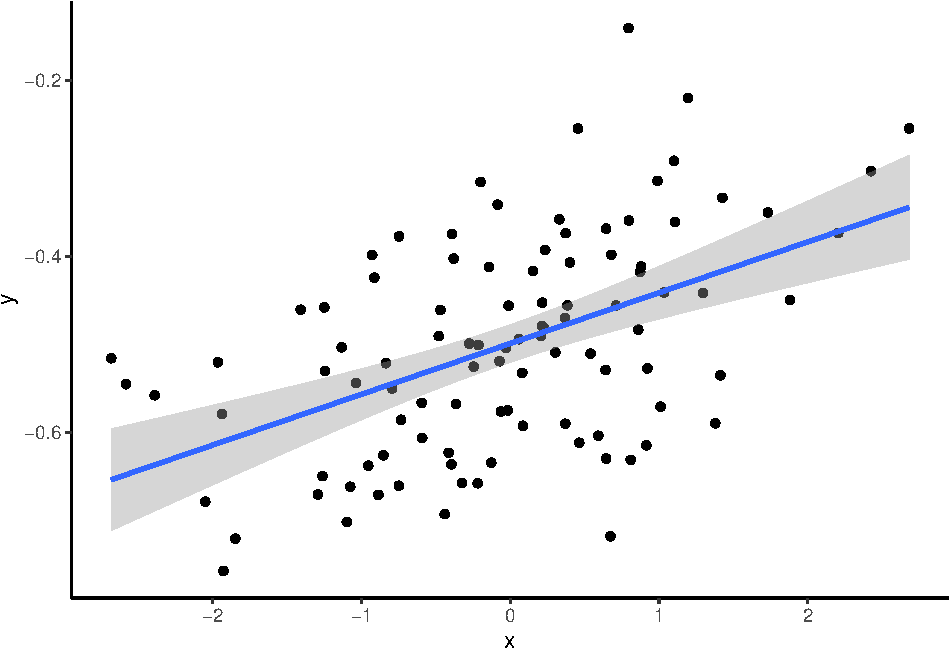
\includegraphics[width=1\linewidth]{_main_files/figure-latex/figS1-1} \caption{Figure caption}\label{fig:figS1}
\end{figure}

\end{document}
